\documentclass{article}
\usepackage[left=1in, right=1in, top=1in, bottom=1in]{geometry}
\usepackage{graphicx}
\usepackage{subfig}
\usepackage{amsmath}

\title{One-trait, three-rate Brownian Motion calibrated validation
  (rate-shift model)}
\author{F\'{a}bio K. Mendes}
\date{March 2019}

\begin{document}
\maketitle

\newpage

\section{Multivariate-normal likelihood class}

Priors for simulations were $\mu \sim \text{N}(0, 2)$, and $\sigma^2 \sim \text{Exp}(5)$. We simulated a single tree (50 tips) from a Yule prior and fixed it.

\begin{figure}[h]
  \centering
  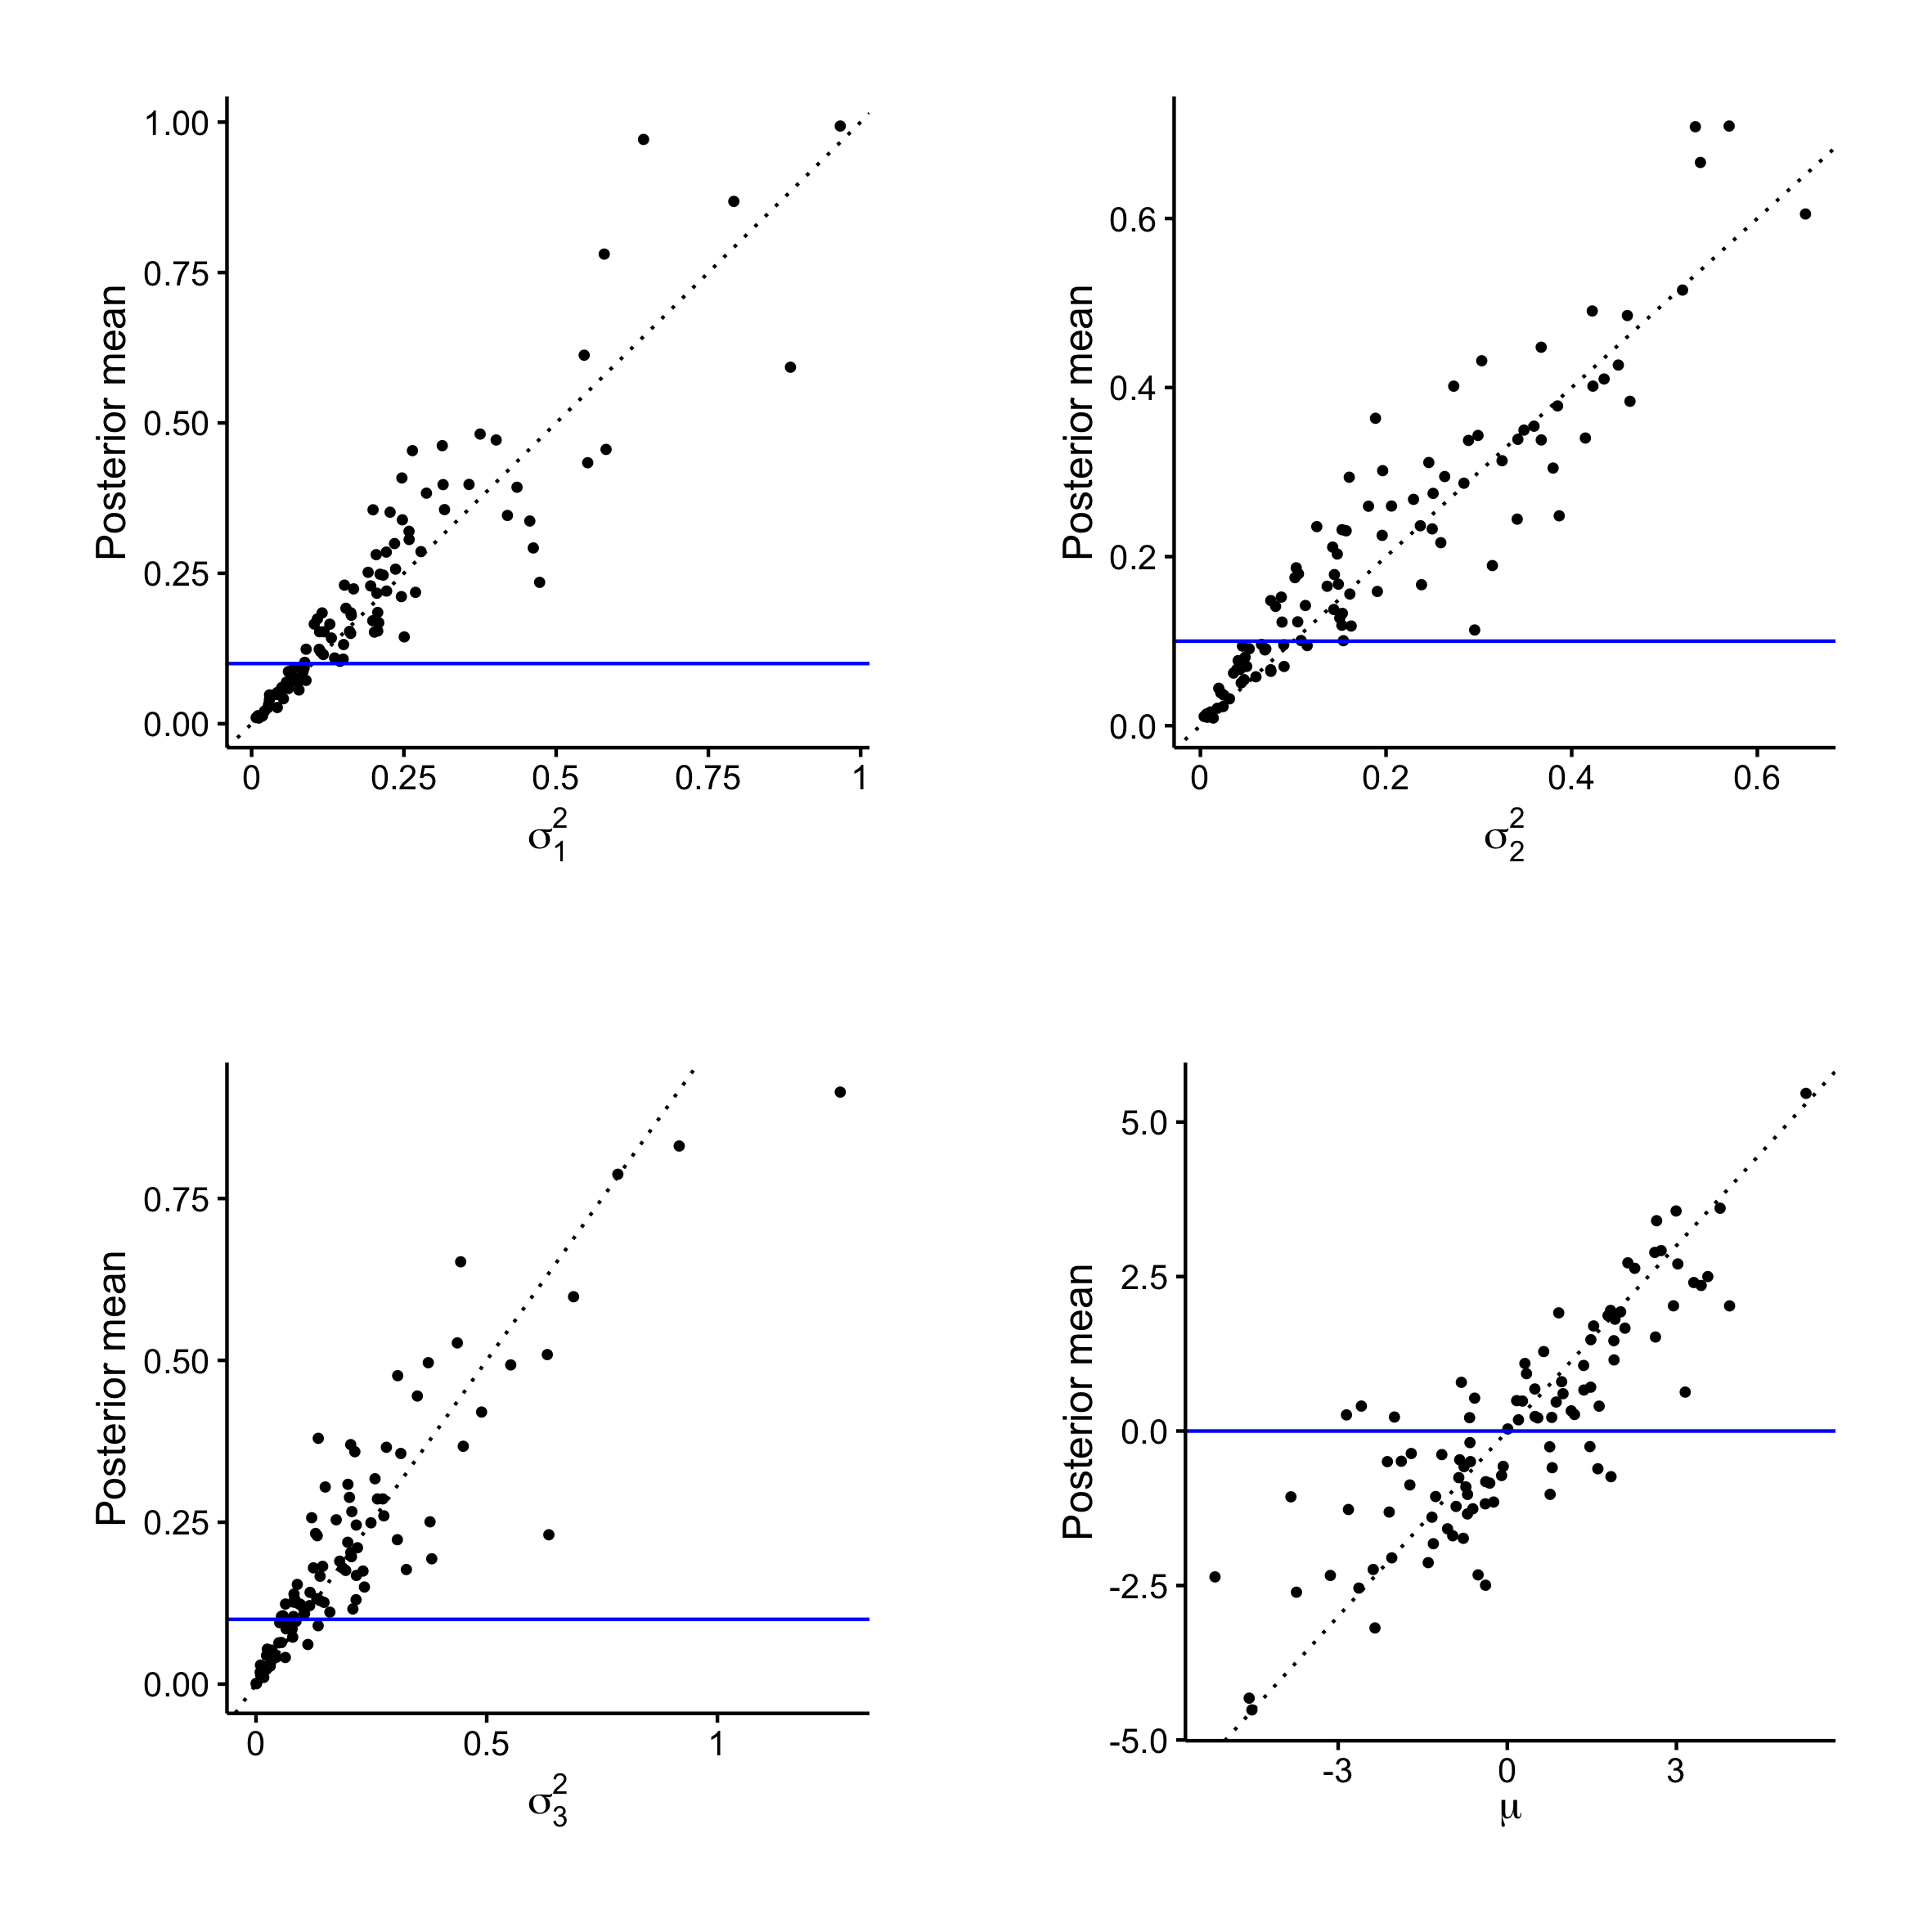
\includegraphics[width=12cm]{../BMMVNShiftThreeRates_ultra_graphs.png}
\end{figure}

\begin{figure}[h]
  \centering
  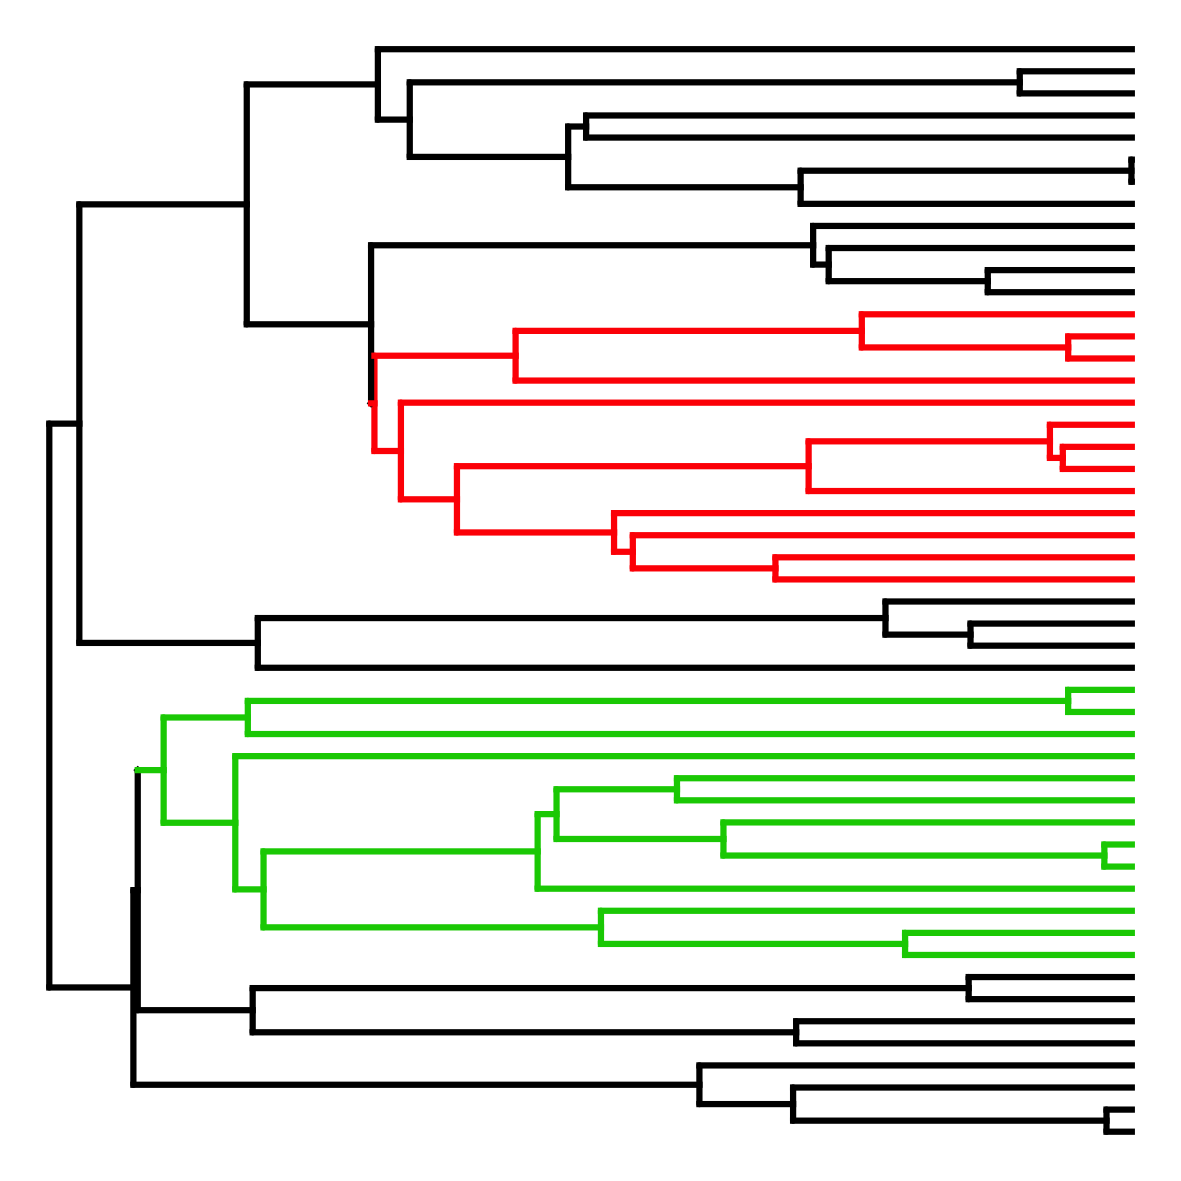
\includegraphics[width=5cm]{../BMMVNShiftThreeRates_ultra_tree.png}
\end{figure}

\begin{center}
\begin{tabular}{c | c}
  Parameter & Coverage (\%) \\\hline
  $\mu$ & 93\\
  $\sigma_1^2$ & 96\\
  $\sigma_2^2$ & 99\\
  $\sigma_3^2$ & 95
\end{tabular}
\end{center}

\newpage

\noindent We re-simulated data on this other tree with approximately half of the tips made short manually (all branch lengths = 0.1).

\begin{figure}[h]
  \centering
  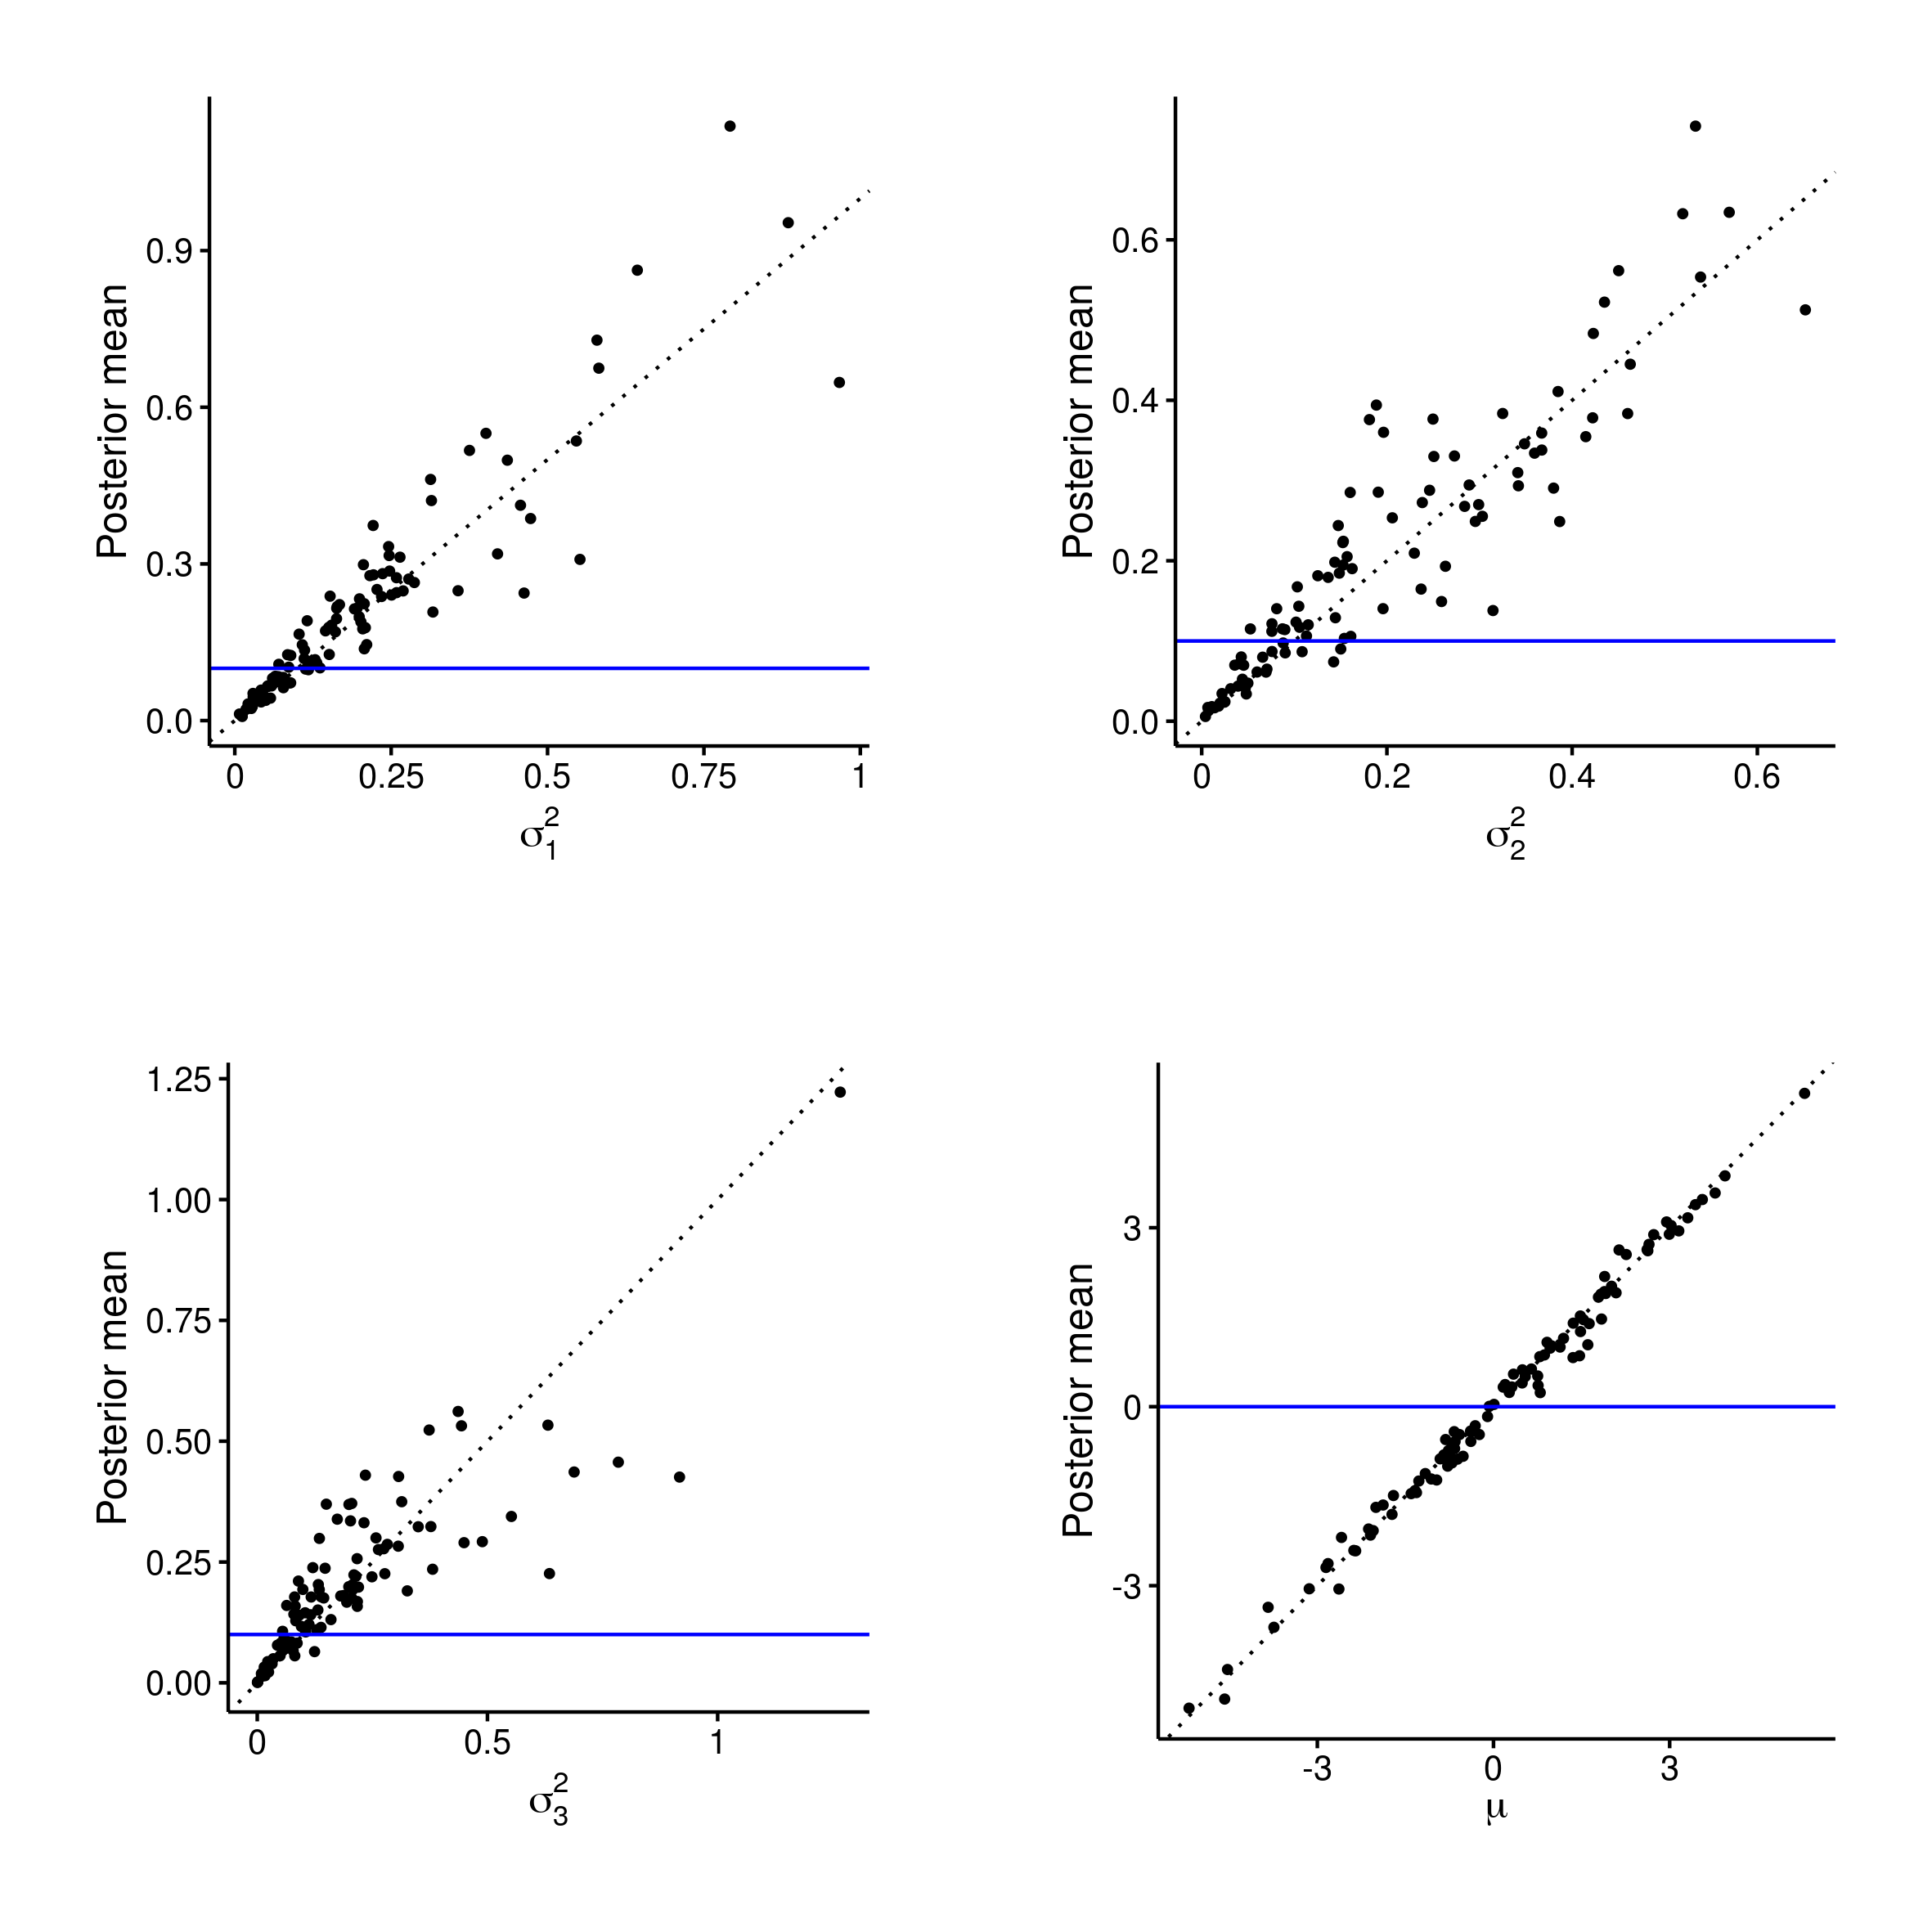
\includegraphics[width=12cm]{../BMMVNShiftThreeRates_nonultra_graphs.png}
\end{figure}

\begin{figure}[h]
  \centering
  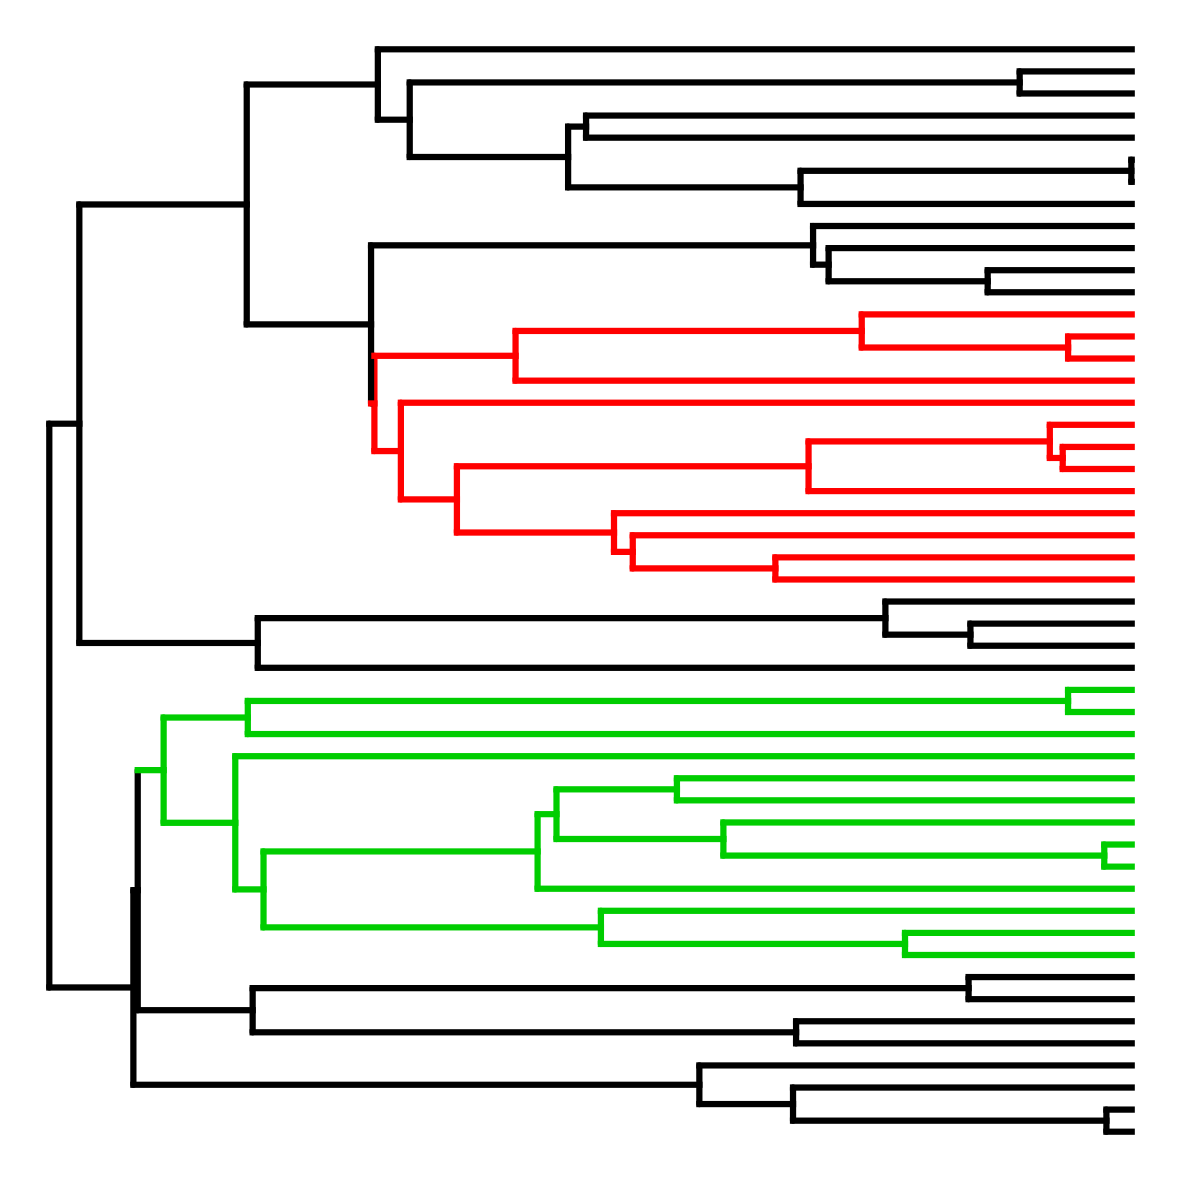
\includegraphics[width=5cm]{../BMMVNShiftThreeRates_nonultra_tree.png}
\end{figure}

\begin{center}
\begin{tabular}{c | c}
  Parameter & Coverage (\%) \\\hline
  $\mu$ & 89\\
  $\sigma_1^2$ & 97\\
  $\sigma_2^2$ & 97\\
  $\sigma_3^2$ & 96
\end{tabular}
\end{center}

\end{document}
